\chapter[Training velociraptors to hoverboard]{Extensive training of velociraptors confirms this was a terrible idea}
\label{chap:velociraptor}

\begin{abstract}
  Here is the chapter abstract.
\end{abstract}

\section{Introduction}

Here is the introduction.

\begin{figure}
  \centering
  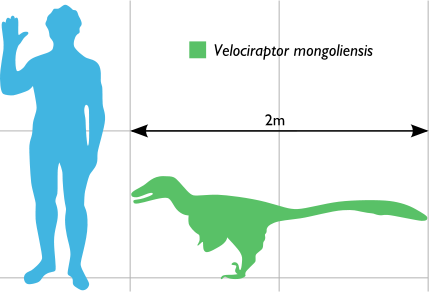
\includegraphics[width=.95\textwidth]{ch3-velociraptor/Velociraptor.png}%Note that this is the path for the folder for chapter 3
  \caption[Velociraptors to scale]{We use only small dinosaurs in these experiments to reduce disembowelment risks.}
  \label{fig:velociraptor}
\end{figure}

\section{Methods}

Let's just say we went through quite a lot of lab techs...

\section{Results}
We briefly present the results of our training; it didn't go so well...

\begin{table}
  \centering
  \caption[Results of dinosaur training]{
    The results showing how many times the three velociraptors were successfully trained, killed someone, or had to be excluded for other reasons.
  }
  \singlespacing
  \begin{tabular}{llrrr}
\toprule
Name & Success & Death & Excluded \\
\midrule
Dinosaur1  &   79 &   63 &  16 \\
Dinosaur2  &  286 &  250 &  36 \\
Dinosaur3  &   89 &   87 &   2 \\
\bottomrule
\end{tabular}
 %this is the .tex file with the table settings in ch3-velociraptor folder
  \label{tab:dinosaur}
\end{table}

\section{Discussion}

Here is the discussion. But we probably won't try this again with carnivorous dinosaurs.
